% das Paket "flashcards" erzeugt Karteikarten zum lernen
% auf der Vorderseite steht das Buzzword oder die Frage
% auf der Rückseite steht die Antwort
% beim ausdrucken auf doppelseitiges Drucken achten
%
\documentclass[avery5371, frame]{flashcards}
\usepackage[utf8]{inputenc}
\usepackage[]{amsmath} 
\usepackage[]{amssymb}
\usepackage{bussproofs} % prooftrees
\usepackage{mdwlist} % less space for lists
\usepackage{graphicx,overpic}
\cardfrontstyle{headings}
\begin{document}
%%%%%%%%%%%%%%%%%%%%%%%%%%%%%%%%%%%%%

\begin{flashcard}{Informationstheoretische Sicherheit des Vernam-Systems} Sei $l>0$ und $S=(X,K,Y,e,d)$ mit $X=K=Y=\{0,1\}^l$ und $e=d=\oplus_l$ das Vernam-System der Länge $l$. Sei weiter $Pr_K:K\rightarrow [0,1]$ die Gleichverteilung. Dann ist $V=S[Pr_K]$ informationstheoretisch sicher.
\end{flashcard}

\begin{flashcard}[Kryptosysteme]{Ein Kryptosystem ist ein Tupel $S=(X,K,Y,e,d)$, wobei}
    \begin{itemize*}
        \item X nicht leere endliche Menge als Klartext
        \item K nicht leere endliche Menge als Schlüssel
        \item Y eine Menge als Chiffretexte
        \item $e:X\times K\rightarrow Y$ Verschlüsselungsfunktion
        \item $d:Y\times K\rightarrow X$ Entschlüsselungsfunktion
    \end{itemize*}
\end{flashcard}

\begin{flashcard}{Ein Kryptosystem mit Schlüsselverteilung (KSV) ist ein 6-Tupel $V=(X,K,Y,e,d,Pr_K)$, wobei}
    \begin{itemize*}
        \item $S=(X,K,Y,e,d)$ das zugrundeliegende Kryptosystem ist
        \item $Pr_K:K\rightarrow (0,1]$ die Schlüsselverteilung
        \item Für $V=(X,K,Y,e,d,Pr_K)$ schreiben wir auch $S[Pr_K]$
        \item $Pr_K(k)\in (0,1]$ also $Pr_K(k)> 0$ für alle $k\in K$
        \item weiter $Pr_X:X\rightarrow [0,1]$ Klartextverteilung
        \item $Pr:X\times K\rightarrow [0,1]$ durch $Pr((x,k)):=Pr_X(x)*Pr_K(k)$
        %\item Annahme modelliert, dass der Schlüssel k unabhängig vom Klartext durch ein von $Pr_K$ gesteuertes Zufallsexperiment gewählt
    \end{itemize*}
\end{flashcard}

\begin{flashcard}[Kryptosysteme]{Dechiffrierbedingung}
    $\forall x\in X\forall k\in K:d(e(x,k),k) =x$
\end{flashcard}

\begin{flashcard}[Kryptosysteme]{Surjektivität}
    $\forall y\in Y\exists x\in X,k\in K:y=e(x,k)$
\end{flashcard}

\begin{flashcard}[Kryptosysteme]{Unter einer Chiffre von $S$ versteht man}
    die Funktion $e(.,k):X\rightarrow Y$, $x\rightarrow e(x,k)$ für festes $k\in K$
\end{flashcard}

\begin{flashcard}[Kryptosysteme]{Ein Kryptosystem heißt possibilistisch sicher, wenn gilt}
    \begin{itemize*}
        \item $\forall y\in Y\forall x\in X\exists k\in K:e(x,k)=y$
        \item Schlüssel mindestens so lang wie der zu übermittelnde Text
        \item in jeder Spalte für $e$ kommen alle Chiffretexte vor
        \item in jeder Zeile für $e$ müssen die Einträge verschieden voneinander sein
    \end{itemize*}
\end{flashcard}

\begin{flashcard}[Kryptosysteme]{Sei $(S,P_k)$ ein Kryptosystem mit Schlüsselverteilung. Es heißt informationstheoretisch sicher bezüglich $Pr_x$, wenn gilt}
    \begin{itemize*}
        \item Eintreten von x und y sind unabhängig
        \item wenn für alle $x\in X,y\in Y$ mit $Pr(y)>0$ gilt: $Pr(x) = Pr(x|y)$.
        %\item $\forall x\in X \forall y\in Y: Pr(x,y)=Pr(x)Pr(y)$
        \item bezüglich jeder beliebigen Klartextverteilung $Pr_X$ informationstheoretisch sicher
        \item $(X,K,Y,e,d)$ ist possibilistisch sicher und $Pr_K(k)=\frac{1}{|K|}$ für alle $k\in K$
        \item in jeder Spalte für $e$ alle Chiffretexte vorkommen und die Schlüsselverteilung $Pr_K$ uniform
        \item für jede Spalte Chiffretextwahrs. separat
    \end{itemize*}
\end{flashcard}

\begin{flashcard}[Definition]{Cäsarchiffe}
    Cäsar ließ Texte verschlüsseln, indem man nimmt immer den Buchstaben, der im Alphabet drei Positionen ,,weiter rechts'' steht, mit ,,wrap around'' am Ende.
\end{flashcard}

\begin{flashcard}[Definition]{Verschiebechiffre}
    Eine Verschiebechiffre ist ein Kryptosystem $S=(Z_n,Z_n,Z_n,e,d)$ mit $e(x,k)=(x+k) mod\ n$

    Verschiebe zyklisch um eine Anzahl k von Buchstaben
\end{flashcard}

\begin{flashcard}[Definition]{Substitutionschiffre}
    Das Bild eines Buchstabens soll ein ganz beliebiger anderer Buchstabe sein. Dabei müssen natürlich verschiedene Buchstaben auf verschiedene Buchstaben abgebildet werden. Es ergibt sich eine Chiffre, die durch eine Tabelle mit ganz beliebiger Buchstabenanordnung gegeben ist.
    Wenn man hier ver- und entschlüsseln möchte, muss man die gesamte zweite Tabellenzeile kennen. Diese kann hier also als ,,Schlüssel'' dienen. Es gibt $21!\approx 5,11* 10^{19}$ viele verschiedene Schlüssel.
\end{flashcard}

\begin{flashcard}[Definition]{Vigenère-Kryptosystem}
    Das Vigenère-Kryptosystem (mit Parametern $(n,S,L)\in\mathbb{N}^3$) ist das Kryptosystem ($(\mathbb{Z}_n)\geq L,(\mathbb{Z}_n)\geq S,(\mathbb{Z}_n)\geq L,e,d$), so dass für alle $s\geq S,l\geq L,x_i,k_j\in\mathbb{Z}_n$ gilt: $e(x_0...x_{l-1},k_0 ...k_{s-1})=y_0 ...y_{l-1}$ mit $y_i=(x_i+k_{i\ mod\ s}) mod\ n$, für alle $0\geq i < l$.
\end{flashcard}

\begin{flashcard}[Definition]{Kasiki Test}
    Die Schlüssellänge kann oft durch den Kasiski-Test näherungsweise bestimmt werden. Stimmt der Klartext im Abschnitt $i+s*l$ bis $j+s*(l+h)$ mit dem Klartext im Abschnitt von $i+s*l'$ bis $j+s*(l'+h)$ überein, so gilt dies auch für den Chiffretext $(1\geq i,j\geq s,l,l',h\in\mathbb{N})$. Kommt ein Teilwort im Klartext an zwei Positionen i und j und ist j-i ein Vielfaches von s, so werden die beiden Vorkommen des Wortes gleich verschlüsselt.
\end{flashcard}

\begin{flashcard}[Definition]{Koinzidenzindex und Friedman-Methode}
    Die Methode beruht darauf, dass die Buchstabenhäufigkeiten fest stehen und sich bei der Verschlüsselung mit einer einfachen Substitutionschiffre nicht ändert. Ebenso ändert sich nicht die Wahrscheinlichkeit, bei der zufälligen Wahl eines Buchstabenpaars zwei identische Buchstaben zu erhalten.
\end{flashcard}

\begin{flashcard}[Definition]{Vernam Kryptosystem}
    Das Vernam-Kryptosystem oder one-time pad der Länge $l$ ist das Kryptosystem $(\{0,1\}^l,\{0,1\}^l,\{0,1\}^l,\oplus_l,\oplus_l)$.
    \begin{enumerate*}
        \item Für $x\in X$ und $k\in K$ gelten $d(e(x,k),k)=(x\oplus_l k)\oplus_l k=x\oplus_l(k\oplus_l k) =x\oplus_l 0^l=x$, d.h. die Dechiffrierbedingung ist erfüllt.
        \item Für $y\in Y$ gilt $e(y,0^l) =y$ und $y\in X,0^l\in K$. Also gilt Surjektivität.
    \end{enumerate*}
\end{flashcard}

\begin{flashcard}[Kryptosysteme]{Kerkoff-Prinzip}
    besagt,dass man davon ausgehen muss, dass Eva die Struktur des Verschlüsselungsverfahrens kennt und die Sicherheit nur von der Geheimhaltung des Schlüssels abhängen darf
\end{flashcard}

\begin{flashcard}[Angriffe]{4 Arten von Angriffsszenarien}
    \begin{description*}
        \item[ciphertext-only attack] (COA) nur mithören
        \item[known-plaintext attack] (KPA) Paare von Klartext und Chiffretext bekannt
        \item[chosen-plaintext attack] (CPA) einige von Eva gewählte Klartexte verschlüsseln
        \item[chosen-cyphertext attack] (CCA) einige von Eva gewählte Chiffretexte entschlüsseln
    \end{description*}
\end{flashcard}

\begin{flashcard}[Block Kryptosystemen]{Beschreibe Szenario 2}
    Alice möchte Bob mehrere verschiedene Klartexte vorher bekannter und begrenzter Länge übermitteln.

    Sie verwendet dafür immer denselben Schlüssel.

    Eva hört die Chiffretexte mit und kann sich sogar einige Klartexte mit dem verwendeten Schlüssel verschlüsseln lassen.
\end{flashcard}

\begin{flashcard}[Block Kryptosysteme]{Nenne ein informationstheoretisch sicheres Block-Kryptosystem, das von Eva in Szenarium 2 leicht gebrochen werden kann.}
    Aus Kenntnis von $x\in\{0,1\}^l$ und $y=e(x,k)$ für ein einziges Paar $(x,k)\in X\times K$ kann Eva den Schlüssel $k=x\oplus_l y$ berechnen. Das gilt für das Cäsar-System, das Vigenère-System und das informationstheoretisch sichere \textbf{Vernam}-System.
\end{flashcard}

\begin{flashcard}{Wann ist ein Kryptosystem possibilistisch sicher bzgl. Szenarium 2}
    Ein Kryptosystem $S=(X,K,Y,e,d)$ ist possibilistisch sicher bzgl. Szenarium 2, wenn für jedes $1 \leq r\leq |X|$, jede Folge von paarweise verschiedenen Klartexten $x_1,x_2,...,x_r\in X$, jeden Schlüssel $k\in K$ und jedes $y\in Y\backslash\{e(x_i,k)| 1 \leq i < r\}$ ein Schlüssel $k'\in K$ existiert mit $e(x_i,k)=e(x_i,k')$ für alle $1\leq i< r$ und $e(x_r,k')=y$.
\end{flashcard}

\begin{flashcard}{Definition l-Block-Kryptosystem}
    Sei $l>0$. Ein l-Block-Kryptosystem ist ein Kryptosystem $S=(\{0,1\}^l,K,\{0,1\}^l,e,d)$ mit $K\subseteq \{0,1\}^s$ für ein $s>0$.
\end{flashcard}

\begin{flashcard}{Ein Substitutions-Permutations-Netzwerk (SPN) ist ein Tupel $N=(m,n,r,s,S,\beta,\kappa)$ wobei}
    \begin{itemize*}
        \item positive ganzen Zahlen $m,n,r$ und $s$ die Wortanzahl, Wortlängen, Rundenzahl und Schlüssellänge
        \item $S:\{0,1\}^n\rightarrow\{0,1\}^n$ eine bijektive Funktion (S-Box)
        \item ${\beta}:\{0,...,mn-1\}\rightarrow\{0,...,mn-1\}$ selbstinverse Permutation (Bitpermutation)
        \item $\kappa :\{0,1\}s\times\{0,...,r\}\rightarrow\{0,1\}^{mn}$ Rundenschlüsselfunktion
    \end{itemize*}
\end{flashcard}

\begin{flashcard}[Ablauf]{Chiffrierung eines Substitutions-Permutations-Kryptosystem}
    für $x\in\{0,1\}^{mn}$ und $k\in\{0,1\}^s$
    \begin{enumerate*}
        \item Initialisierung: $u=x\oplus_{mn} \kappa (k,0)$.
        \item Verschlüsselung in Runden für $i=1,...,r-1$
        \begin{enumerate*}
            \item $v(j)=S(u(j))$ für $0\leq j<m$ (jedes Wort einzeln durch die S-Box)
            \item $w=v^{\beta}$ (Bitpermutation auf Gesamtwort)
            \item $u=w\oplus_{mn} \kappa (k,i)$ (XOR mit Schlüssel)
            \item Schlussrunde $v(j)=S(u(j))$ für $0\leq j<m$
            \item Ausgabe: $y=v\oplus \kappa (k,r)$
        \end{enumerate*}
    \end{enumerate*}
\end{flashcard}

\begin{flashcard}[Definition]{AES - Advanced Encryption Standard}
    \begin{itemize*}
        \item ist ein symmetrisches Verschlüsselungsverfahren
        \item die Klartextlänge und Chiffretextlänge stets $l= 128$
        \item die Schlüssellänge $128,192$ oder $256$ Bits
        \item Arithmetik im Körper $GF(2^8)$ benutzt, dessen Elemente $8$-Bit-Vektoren, also Bytes, entsprechen
    \end{itemize*}
\end{flashcard}

\begin{flashcard}[Block Kryptosysteme]{In der Vorlesung wurde possibilistische Sicherheit für Szenarium 2 definiert. Nenne ein $l$-Block-Kryptosystem, das diese Definition erfüllt. Die nötige Schlüsselmenge $K$ hat Größe\dots}
    Ein Kryptosystem $S=(X,K,Y,e,d)$ ist possibilistisch sicher bzgl. Szenarium 2, wenn für jedes $1 \leq r\leq |X|$, jede Folge von paarweise verschiedenen Klartexten $x_1,x_2,\dots,x_r\in X$, jeden Schlüssel $k\in K$ und jedes $y\in Y\backslash\{e(x_i,k)| 1 \leq i < r\}$ ein Schlüssel $k'\in K$ existiert mit $e(x_i,k)=e(x_i,k')$ für alle $1\leq i< r$ und $e(x_r,k')=y$.

    Die nötige Schlüsselmenge $K$ hat Größe $\frac{|Y|!}{(|Y|-|X|)!} \geq |X|!$ viele Schlüssel.
    Mit $X=\{0,1\}^{128}$  gibt es also $\geq 2^{128}!$ viele Schlüssel.
\end{flashcard}

\begin{flashcard}[Block Kryptosysteme]{Nenne ein Block-Kryptosystem aus der Vorlesung, das gegenwärtig für Szenarium 2 in der Praxis benutzt wird.}
    AES
\end{flashcard}

\begin{flashcard}[Block Kryptosysteme]{Beschreibe das Konzept eines $l$-Unterscheiders}
    Ein l-Unterscheider ist ein randomisierter Algorithmus $U(F:\{0,1\}^l\rightarrow\{0,1\}^l):\{0,1\}$, dessen Laufzeit bzw. Ressourcenaufwand durch eine Konstante beschränkt ist.
    %Das Argument des l-Unterscheiders ist eine Chiffre $F$. Diese ist als ,,Orakel'' gegeben, das heißt als Prozedur, die nur ausgewertet werden kann, deren Programmtext $U$ aber nicht kennt. Das Programm $U$ kann $F$ endlich oft aufrufen, um sich Paare zu besorgen. Danach kann $U$ noch weiter rechnen, um zu einer Entscheidung zu kommen. Das von $U$ gelieferte Ergebnis ist ein Bit.
    Für ein gegebenes Block-Kryptosystem $B$ ist das gewünschte Verfahren: Programm $U$ sollte 1 liefern, wenn $F$ eine Chiffre $e(.,k)$ zu $B$ ist, und $0$, wenn $F=\pi$ für eine Permutation $\pi\in P\{0,1\}^l$ ist, die keine $B$-Chiffre ist.
\end{flashcard}

\begin{flashcard}[Block Kryptosysteme]{Beschreibe das zugehörige Sicherheitsspiel eines $l$-Unterscheiders}
    Man entscheidet mit einem Münzwurf, ob Unterscheider $U$ für seine Untersuchungen als $F(.)$ eine zufällige Chiffre $e(.,k)$ von Kryptosystem $B$ oder eine zufällige Permutation $\pi$ von $\{0,1\}^l$ erhalten soll. Dann rechnet $U$ mit $F$ als Orakel und gibt dann seine Meinung ab, ob er sich in der Realwelt oder in der Idealwelt befindet. U ,,gewinnt'', wenn diese Meinung zutrifft.
\end{flashcard}

\begin{flashcard}[Block Kryptosysteme]{Definiere den Vorteil eines $l$-Unterscheiders.}
    \begin{itemize*}
        \item der Vorteil von $U$ bzgl. $B$ ist $adv(U,B):= 2(Pr(G^B_U=1)-\frac{1}{2})$
        \item Für jeden l-Unterscheider $U$ und jedes l-Block-KS $B$ gilt $-1\geq adv(U,B)\geq 1$
        \item Werte $adv(U,B)<0$ sind uninteressant (Ausgaben können vertauscht werden um positiven Vorteil zu erhalten)
    \end{itemize*}
\end{flashcard}

\begin{flashcard}{Ein symmetrisches $l$-Kryptoschema ist ein Tupel $S= (K,E,D)$, wobei}
    \begin{itemize*}
        \item $K\subseteq\{0,1\}^s$ endliche Menge (für ein $s\in\mathbb{N}$)
        \item $E(x:\{0,1\}^{l*},k:K) :\{0,1\}^{l*}$ randomisierter Algorithmus
        \item $D(y:\{0,1\}^{l*},k:K) :\{0,1\}^{l*}$ deterministischer Algorithmus
        \item Laufzeiten von $E$ und $D$ sind polynomiell beschränkt in der Länge von $x$ bzw. $y$
        \item Dechiffrierbedingung: $\forall x\in\{0,1\}^{l*},k\in K,m\in M_1\times...\times M_r$ gilt: $D(E^m(x,k),k)=x$
    \end{itemize*}
\end{flashcard}

\begin{flashcard}[Betriebsarten]{Beschreibe die ECB-Betriebsart (Electronic Code Book)}
    Ein Schlüssel ist ein Schlüssel $k$ von $B$. Man verschlüsselt einfach die einzelnen Blöcke von $x$ mit $B$, jedes mal mit demselben Schlüssel $k$.
    %Es wird nicht $x_i$ mit $B$ verschlüsselt, sondern $x_i\oplus_l y_{i-1}$ (bitweises XOR). Man benötigt dann einen Anfangsvektor $y_{-1}$ für die erste Runde. Dieser ist Teil des Schlüssels des Kryptoschemas (nicht von B), ein Schlüssel des Schemas ist also ein Paar $(k,v)$ mit $k\in K_B$ und $v\in\{0,1\}^l$.

    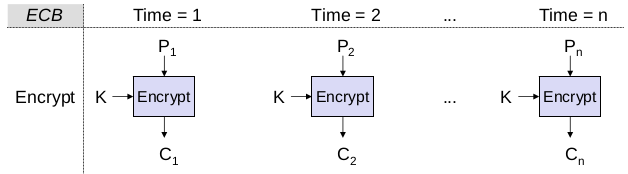
\includegraphics[width=.9\linewidth]{Assets/NetworkSecurity-electronic-code-book-mode.png}
\end{flashcard}

\begin{flashcard}[Betriebsarten]{Beschreibe die CBC-Betriebsart (Cipher Block Chaining)}
    Blöcke in Runden $i=0, 1 ,\dots,m-1$ nacheinander verschlüsselt und das Ergebnis einer Runde wird zur Modifikation des Klartextblocks der nächsten Runde benutzt.

    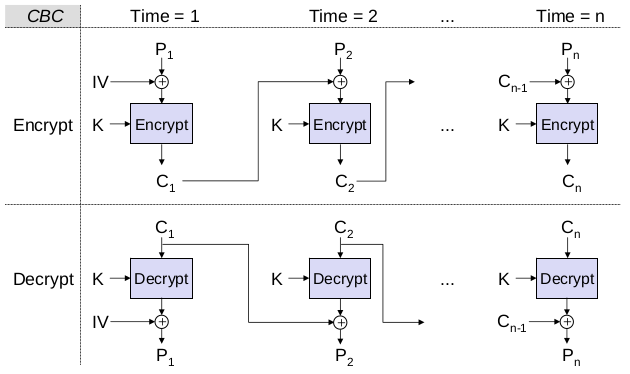
\includegraphics[width=.6\linewidth]{Assets/NetworkSecurity-cipher-block-chaining-mode.png}
\end{flashcard}

\begin{flashcard}[Betriebsarten]{Beschreibe die R-CBC-Betriebsart (Randomized Cipher Block Chaining)}
    Der Initialisierungsvektor $y_{-1}=v\in\{0,1\}^l$ ist nicht mehr Teil des Schlüssels, sondern wird vom Verschlüsselungsalgorithmus einfach zufällig gewählt, und zwar für jeden Klartext immer aufs Neue. Damit der Empfänger entschlüsseln kann, benötigt er $v$. Daher wird $y_{-1}$ als Zusatzkomponente dem Chiffretext vorangestellt. Damit ist der Chiffretext um einen Block länger als der Klartext, und Eva kennt auch $v=y_{-1}$.
\end{flashcard}

\begin{flashcard}[Betriebsarten]{Beschreibe die OFB-Betriebsart (Output FeedBack)}
    Man setzt $k_{-1}=v$, und konstruiert die Rundenschlüssel $k_0,...,k_{m-1}$ durch iterieren des letzten Rundenschlüssel durch die Verschlüsselungsfunktion von $B$: $k_i=e_B(k_{i-1}, k)$%, für $i=0,1,...,m-1$. 
    %Der Empfänger benötigt $v$, um seinerseits die Rundenschlüssel zu berechnen, daher wird $v$ als $y_{-1}$ dem Chiffretext vorangestellt.

    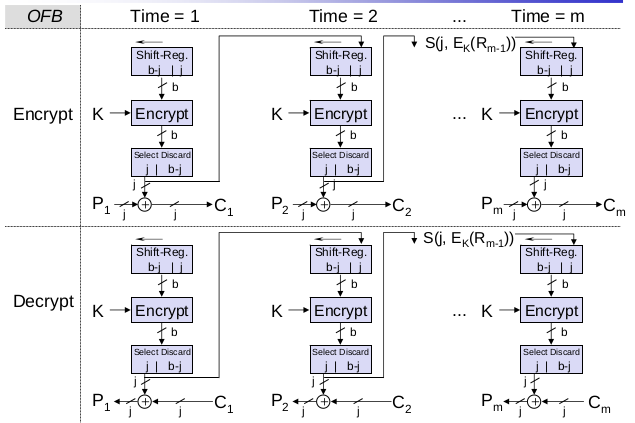
\includegraphics[width=.5\linewidth]{Assets/NetworkSecurity-output-feedback-mode.png}
\end{flashcard}

\begin{flashcard}[Betriebsarten]{Beschreibe die R-CTR-Betriebsart (Randomized CounTeR)}
    Man fasst $\{0,1\}^l$ als äquivalent zur Zahlenmenge $\{0,1,...,2^{l-1}\}$ auf, interpretiert einen $l$-Bit-String also als Block oder als Zahl, wie es passt. In dieser Menge wählt man eine Zufallszahl $r$. Man ,,zählt'' von $r$ ausgehend nach oben und berechnet die Rundenschlüssel $k_0,...,k_{m-1}$ durch Verschlüsseln von $r,r+1,...,r+m-1$ (modulo $2^l$ gerechnet) mittelse $B(.,k)$. Rundenschlüssel $k_i$ ist also $e_B((r+i) mod\ 2^l,k)$, und Chiffretextblock $y_i$ ist $k_i\oplus_l x_i$.
\end{flashcard}

\begin{flashcard}[Betriebsarten]{Nutze die ECB-Betriebsart. Gebe einen Angreifer an, der die Chiffretexte zweier selbstgewählter Klartexte ohne Kenntnis des Schlüssels unterscheiden kann.}
    Ein Block $x\in\{0,1\}^l$ wird immer gleich verschlüsselt. Eva kann also ganz leicht nicht-triviale Informationen aus dem Chiffretext erhalten.
    Zum Beispiel kann sie sofort sehen, ob der Klartext die Form $x=x_1 x_1$, mit $x_1\in\{0,1\}^l$, hat oder nicht.
\end{flashcard}

\begin{flashcard}[Betriebsarten]{Nutze die CBC-Betriebsart. Gebe einen Angreifer an, der die Chiffretexte zweier selbstgewählter Klartexte ohne Kenntnis des Schlüssels unterscheiden kann.}
    Wird zweimal der Klartext $x$ verschlüsselt, so geschieht dies immer durch denselben Chiffretext $y=E(x,(k,v))$. Dies ist eine Folge der Eigenschaft von CBC, deterministisch zu sein.
\end{flashcard}

\begin{flashcard}{Sei $n,q,t,l\in\mathbb{N}$, $A$ ein l-Angreifer, $S$ ein symmetrisches l-Kryptoschema. Dann heißt $A(n,q,t)$-beschränkt, wenn\dots }
    ...die Laufzeit des Experiments $G^S_A$ durch $t$ beschränkt ist, der Algorithmus $H$ (als Orakel) höchstens $q$ mal aufgerufen wird und bei diesen Aufrufen höchstens $n$ Blöcke verwendet werden.
\end{flashcard}

\begin{flashcard}[Zahlentheorie]{Auf Eingabe $x,y\in\mathbb{N}$ liefert der Euklidische Algorithmus eine ganze Zahlen $d$ mit \dots}

    \begin{itemize*}
        \item[] $a,b:integer;a\leftarrow |x|;b\leftarrow |y|;$
        \item[] $while\ b> 0\ repeat$
        \begin{itemize*}
            \item[] $(a,b)\leftarrow (b,a\ mod\ b);$ %// simultane Zuweisung
        \end{itemize*}
        \item[] return $a$
    \end{itemize*}

    Der Euklidische Algorithmus liefert eine ganze Zahl $d$, die der größte gemeinsame Teiler von $x$ und $y$ ist.
\end{flashcard}

\begin{flashcard}[Zahlentheorie]{Auf Eingabe $x,y\in\mathbb{N}$ liefert der erweiterte Euklidische Algorithmus (EEA) drei ganze Zahlen $d,s,t$.

        Welche Eigenschaften erfüllen diese?}

    \begin{enumerate*}
        \item Für die Ausgabe $(d,s,t)$ gilt $d= ggT(x,y) =s*x+t*y$.
        \item Die Anzahl der Schleifendurchläufe ist dieselbe wie beim gewöhnlichen Euklidischen Algorithmus
        \item Die Anzahl von Ziffernoperationen ist $O((log\ x)(log\ y))$
    \end{enumerate*}
\end{flashcard}

\begin{flashcard}[Zahlentheorie]{Wenn er auf zwei Zahlen mit je $n$ Bits angewendet wird, führt der erweiterte Euklidische Algorithmus $O(\dots)$ Bitoperationen aus.}
    $O((log\ x)(log\ y))$
\end{flashcard}

\begin{flashcard}[Zahlentheorie]{Seien $a$ und $N$ teilerfremde natürliche Zahlen. Wie kann man eine ganze Zahl $b$ ermitteln, die die Gleichung $a*b\ mod\ N= 1$ erfüllt?}

    $(a*b)\ mod\ N = (a\ mod\ N * b\ mod\ N)mod\ N = 1$
\end{flashcard}

\begin{flashcard}[Zahlentheorie]{Gebe den Algorithmus der Funktion $modexp(x,y,N)$ zur rekursiven Berechnung von $x^y\ mod\ n$ mithilfe der schnellen modularen Exponentiation an.

        Dieser Algorithmus führt $O(\dots)$ modulare Multiplikationen aus.}

    function $modexp(x,y,m)$
    \begin{itemize*}
        \item[] if $y= 0$ then return $1$
        \item[] if $y= 1$ then return $x$
        \item[] $z\leftarrow modexp((x*x) mod\ m,\lfloor y/2\rfloor,m);$ %// rekursiver Aufruf
        \item[] if $y$ ist ungerade then $z\leftarrow (z*x) mod\ m$
        \item[] return $z$
    \end{itemize*}

    erfordert $O((log\ m)^2)$ Ziffernoperationen
\end{flashcard}

\begin{flashcard}[Zahlentheorie]{Vervollständige den Chinesischen Restsatz:

        Wenn $m$ und $n$ \dots Zahlen sind, dann ist die Abbildung $\Phi:\dots\rightarrow\dots, x\rightarrow \dots,\dots$.}
    Wenn $m$ und $n$ teilerfremde Zahlen sind, sind die Strukturen $\mathbb{Z}_m \times\mathbb{Z}_n$ und $\mathbb{Z}_{mn}$ isomorph.

    Dann ist die Abbildung $\Phi:\mathbb{Z}_{mn} \owns x \rightarrow (x\ mod\ m, x\ mod\ n)\in\mathbb{Z}_m\times\mathbb{Z}_n$ bijektiv. Weiterhin: Wenn $\Phi(x)=(x_1,x_2)$ und $\Phi(y)=(y_1,y_2)$, dann gilt:
    \begin{itemize*}
        \item $\Phi(x+_{mn} y) = (x_1 +_m y_1 , x_2 +_n y_2)$
        \item $\Phi(x*_{mn} y) = (x_1 *_m y_1 , x_2 *_n y_2)$
        \item $\Phi(1) = (1,1)$
    \end{itemize*}
\end{flashcard}

\begin{flashcard}[Zahlentheorie]{Vervollständige den kleinen Satz von Fermat:

        Wenn $p$ \dots ist und $a$ in \dots liegt, dann gilt: \dots}
    Wenn $p$ eine Primzahl ist und $a\in\mathbb{Z}^*_p$ liegt,

    dann gilt $a^{p-1}\ mod\ p= 1$
\end{flashcard}

\begin{flashcard}[Zahlentheorie]{ Vervollständige den Satz von Euler:

        Für $m\geq 2$ und $x$ mit \dots gilt \dots .}
    Für $m\geq 2$ und $x$ mit $ggT(m,x) = 1$ gilt $x\varphi(m)\ mod\ m=1$
\end{flashcard}

\begin{flashcard}[Primzahlen]{Definiere den Begriff ,,$a$ ist ein F-Lügner'' (für $N$):

        $N$ ist \dots und es gilt \dots .}
    Sei $N\geq 3$ ungerade und zusammengesetzt.

    Eine Zahl $a\in\{1,\dots,N-1\}$ heißt \textbf{F-Zeuge} für $N$, wenn $a^{N-1} mod\ N\not= 1$ gilt.

    Eine Zahl $a\in\{1,\dots,N-1\}$ heißt \textbf{F-Lügner} für $N$, wenn $a^{N-1} mod\ N=1$ gilt.

    Die Menge der F-Lügner nennen wir $L^F_N$.
\end{flashcard}

\begin{flashcard}[Primzahlen]{$N$ heißt Carmichael-Zahl, wenn \dots}
    Eine ungerade zusammengesetzte Zahl $N$ heißt eine Carmichael-Zahl, wenn für alle $a\in\mathbb{Z}^*_N$ die Gleichung $a^{N-1}\ mod\ N= 1$ gilt.
\end{flashcard}

\begin{flashcard}[Primzahlen]{Formuliere den Fermat-Test für eine gegebene ungerade Zahl $N\geq 5$: Wähle\dots und berechne $c=\dots$. Wenn $c=\dots$ ist, ist die Ausgabe \dots., sonst ist sie \dots .}
    Nutze den Fermat-Test, um ,,Zeugen'' dafür anzugeben, dass eine Zahl $N$ zusammengesetzt ist: Wenn wir eine Zahl $a$ mit $1\leq a < N$ finden, für die $a^{N-1} mod\ N\not=1$ gilt, dann ist $N$ definitiv keine Primzahl.

    Für eine gegebene ungerade Zahl $N\geq 5$: Wähle $a<5$ und berechne $c=a^{N-1}\ mod\ N$. Wenn $c\not=1$ ist, ist die Ausgabe N ist kine Primzahl, sonst ist sie eine Primzahl.
\end{flashcard}

\begin{flashcard}[Primzahlen]{Definiere: $b\in\{1,\dots,N-1\}$ heißt nichttriviale Quadratwurzel der 1 modulo $N$, wenn\dots}
    Eine Zahl $b\in\{2,\dots,N-2\}$ mit $b^2\ mod\ N=1$ heißt eine nicht triviale Quadratwurzel der $1$ modulo $N$. Bei Primzahlen gibt es solche Zahlen nicht.
\end{flashcard}

\begin{flashcard}[Primzahlen]{Wenn man eine nichttriviale Quadratwurzel $b$ der 1 modulo $N$ gefunden hat, weiß man sicher, dass $N$\dots. ist.}
    Wenn es eine nichttriviale Quadratwurzel der $1$ modulo $N$ gibt, dann ist $N$ zusammengesetzt.
\end{flashcard}

\begin{flashcard}[Primzahlen]{Definiere den Begriff $\{$qqa ist ein MR-Lügner$\}$ (für $N$):

        Suche ungerades $u$ und $k\geq 1$ mit\dots=\dots .
        Bilde die Folge $b_0=\dots,b_1=\dots,\dots,b_k=\dots$.
        $a$ heißt dann ein MR-Lügner (für $N$), falls \dots}

    Wir schreiben $N-1=u*2^k$, für $u$ ungerade, $k\geq 1$.

    Eine Zahl $a, 1\leq a < N$, heißt ein MR-Lügner für $N$, wenn $b_0=1$ oder in der Folge $b_0,\dots,b_{k-1}$ zu $a$ kommt $N-1$ vor gilt, $a^u\equiv 1$ oder $a^{u*2^i}\equiv N-1 (mod\ N)$ für ein $i$ mit $0\leq i < k$
\end{flashcard}

\begin{flashcard}[Primzahlen]{Ergänze den Algorithmus von Miller/Rabin (Eingabe $N\geq 5$)}
    \begin{itemize*}
        \item[] suche $u$ ungerade und $k\geq 1$ mit $N-1 =u*2^k$
        \item[] wähle zufällig ein $a$ aus $\{1 ,\dots,N-1\}$
        \item[] $b \leftarrow a^u\ mod\ N$ %// mit schnellem Potenzieren
        \item[] if $b\in\{1,N-1\}$ then return $0$
        \item[] for $j$ from $1$ to $k-1$ do %//,,wiederhole (k-1)-mal''
        \begin{itemize*}
            \item[] $b\leftarrow b^2\ mod\ N$
        \end{itemize*}
        \item[] if $b=N-1$ then return $0$
        \item[] if $b=1$ then return $1$
        \item[] return $1$
    \end{itemize*}
\end{flashcard}

\begin{flashcard}[Primzahlen]{Was kann man über das Ein-/Ausgabeverhalten des Miller-Rabin-Algorithmus auf Eingabe $N\geq 5$ (ungerade) sagen?

        $N$ zusammengesetzt $\Rightarrow$ \dots,

        $N$ Primzahl $\Rightarrow$\dots}
    Wenn $N$ zusammengesetzt $\Rightarrow$ gibt es MR-Zeugen.

    Wenn $N$ eine Primzahl ist, gibt der MR-Test $0$ aus.
\end{flashcard}

\begin{flashcard}[Primzahlen]{Wie kann man vorgehen,

        um aus dem Miller-Rabin-Test einen Primzahltest zu erhalten,

        dessen Fehlerwahrscheinlichkeit höchstens $1/4^l$ beträgt?}
    Tatsächlich ist die Fehlerwahrscheinlichkeit durch $1/4^l$ beschränkt. Dies kann man aber nur durch fortgeschrittene zahlentheoretische Untersuchungen über die erwartete Wahrscheinlichkeit, dass eine zufällige ungerade zusammengesetzte Zahl den $l$-fach iterierten MiRa-Test übersteht, beweisen.
\end{flashcard}

\begin{flashcard}[Primzahlen]{Formuliere den Primzahlsatz}
    Primzahlsatz: $lim_{x\rightarrow \infty} \frac{\pi(x)}{x\backslash ln\ x}= 1$.

    Mit $\pi(x)$ bezeichnen wir die Anzahl der Primzahlen, die nicht größer als $x$ sind.
\end{flashcard}

\begin{flashcard}[Primzahlen]{Nach der Ungleichung von Finsler gibt es $\Omega(\dots)$ Primzahlen im Intervall $[m, 2m)$. Entsprechend muss man für $\mu\in\mathbb{N}$ erwartet nur $O(\dots)$ Zahlen zufällig aus $[2^{\mu-1}, 2^{\mu})$ ziehen, um mindestens eine $\mu$-Bit Primzahl zu erhalten.}
                    Ungleichung von Finsler: Für jede ganze Zahl $m\geq 2$ liegen im Intervall $(m, 2m]$ mindestens $m/(3\ ln(2m))$ Primzahlen: $\pi (2m)-\pi(m)\geq \frac{m}{3\ ln(2m)}$.

    $\Rightarrow \pi(2m)-\pi(m) = O(m/log\ m)$
\end{flashcard}

\begin{flashcard}[Primzahlen]{Zu gegebenem $\mu$ soll eine (zufällige) Primzahl im Intervall $[2^{\mu-1}, 2^{\mu})$ gefunden werden. Wie geht man vor?}
    wiederhole: \dots
    bis Ergebnis \dots erscheint.
    Wie lässt sich die erwartete Anzahl von Bitoperationen für das Finden einer solchen Primzahl abschätzen? $O(\dots)$.
\end{flashcard}

\begin{flashcard}{Ein Public-Key-Kryptosystem $(X,Y,K,E,D)$ hat 5 Komponenten}
    \begin{itemize*}
        \item Klartextmenge $X$ (endlich),
        \item Chiffretextmenge $Y$ (endlich),
        \item Schlüsselmenge $K$, wobei $K\supseteq K_{pub} \times K_{priv}$ für Mengen $K_{pub}$ und $K_{priv}$,
        \item Verschlüsselungsfunktion $E:X\times K_{pub} \rightarrow Y$,
        \item Entschlüsselungsfunktion $D:Y\times K_{priv} \rightarrow X$,
        \item mit Dechiffrierbedingung: $D(E(x,k), \hat{k}) =x$, für alle $x\in X,(k,\hat{k})\in K$.
    \end{itemize*}
\end{flashcard}

\begin{flashcard}{Ein asymmetrisches Kryptoschema ist ein Tupel $S= (X,K,G,E,D)$, wobei}
    \begin{itemize*}
        \item $X,K\supseteq K_{pub} \times K_{priv}$ Mengen,
        \item $G():K_{pub} \times K_{priv}$ randomisierter Algorithmus
        \item $E(x:X,k:K_{pub}):\{0,1\}^*$ randomisierter Algo.
        \item $D(y:\{0,1\}^*,k:K_{priv}):\{0,1\}^*$ determ. Algo.
        \item Laufzeit ist beschränkt durch eine Konstante,
        \item die Laufzeiten von $E$ und $D$ sind polynomiell beschränkt
        \item $\forall x\in X,k\in K_{pub}$ gilt: $D(E^m (x,k),\hat{k}) =x$.
    \end{itemize*}
\end{flashcard}

\begin{flashcard}{ Sei $t\in\mathbb{N}$, $A$ ein Angreifer auf ein asymmetrisches Kryptoschema $S$. Dann heißt $A$ $t$-beschränkt, wenn }
    die Laufzeit des Experiments $G^S_A$ durch $t$ beschränkt ist.
\end{flashcard}

\begin{flashcard}{Sei $\epsilon >0$. Dann heißt $S(t,\epsilon)$-sicher, wenn }
    für jeden $t$-beschränkten Angreifer $A$ gilt $adv(A,S)\leq \epsilon$.
\end{flashcard}

\begin{flashcard}[RSA-System]{Schlüsselerzeugung: Wähle \dots und berechne $N=\dots$ sowie $\varphi(N)=\dots$. Der öffentliche Schlüssel von Bob ist $(N,e)$, wobei $e$ die Bedingung \dots erfüllt. Der geheime Schlüssel von Bob ist $(N,d)$, mit \dots. $d$ lässt sich mit folgendem Algorithmus berechnen: \dots}

    Wähe zwei Primzahlen $p$ und $q$, deren Bitlänge 1/2 der Schlüssellänge ist und das Produkt $N=pq$ sowie $\varphi(N)=(p-1)(q-1)$ berechnet.
    Es wird eine Zahl $e\in\{3,\dots,\varphi(N)-1\}$ mit $ggT(e,\varphi(N)) = 1$ gewählt.
    %Dann wird das multiplikative Inverse $d<\varphi(N) modulo\ \varphi(N)$ von $e$ bestimmt, so dass also $ed\ mod\ \varphi(N) = 1$ gilt.

    \begin{itemize*}
        \item öffentlicher Schlüssel $k$ ist das Paar $(N,e)$
        \item geheimer Schlüssel $\hat{k}$ ist $(N,d)$ mit multiplikativ Inversen $d<\varphi(N) modulo\ \varphi(N)$ von $e$
        \item es gilt $ed\ mod\ \varphi(N) = 1$
        \item Berechnungsaufwand $O((log\ N)^4) =O(l^4)$
    \end{itemize*}
\end{flashcard}

\begin{flashcard}[RSA-System]{Verschlüsseln von $x\in \dots :y=\dots $.}
    $x\in X= [N]: y=E(x,(N,e)) :=x^e\ mod\ N$

    (Zu berechnen mit schneller Exponentiation, Rechenzeit $O((log\ N)^3) =O(l^3)$)
\end{flashcard}

\begin{flashcard}[RSA-System]{Entschlüsseln von $y\in \dots :z=\dots $.}
    $y\in Y: z=D(y,(N,d)) :=y^d\ mod\ N$

    (Zu berechnen mit schneller Exponentiation, Rechenzeit $O((log\ N)^3) =O(l^3)$)
\end{flashcard}

\begin{flashcard}[RSA-System]{Formuliere die zentrale Korrektheitsaussage des RSA-Systems: \dots=$x$, für alle zulässigen Klartextblöcke $x$.}
    Korrektheit/Dechiffrierbedingung von RSA: Wenn $ed\ mod\ \varphi(N) = 1$ gilt, dann haben wir $x^{ed}\ mod\ N=x$, für alle $x\in [N]$.
\end{flashcard}

\begin{flashcard}[RSA-System]{Beschreibe eine Strategie für RSA-basierte Systeme, mit der verhindert werden kann, dass zwei identische Klartextblöcke bei Verwendung desselben Schlüsselpaars gleich verschlüsselt werden.}
    Es ist Empfohlen, beim Arbeiten mit RSA den Klartext $x$ durch das Anhängen eines nicht ganz kurzen Zufallsstrings zu randomisieren. Wenn dieser angehängte Zufallsstring die gleiche Länge wie $x$ hat, ist der Chiffretext genauso lang wie bei ElGamal.
\end{flashcard}

\begin{flashcard}[Rabin-Kryptosystem]{Komponenten des Rabin-Kryptosystems: Zwei große Primzahlen $p$ und $q$ mit \dots . Der öffentliche Schlüssel ist $N=$\dots, der private Schlüssel von Bob ist \dots .}
    Wähle zwei verschiedene zufällige große Primzahlen $p$ und $q$ mit $p\equiv q\equiv 3 (mod\ 4)$, also Primzahlen, die um 1 kleiner als ein Vielfaches von 4 sind. Berechne $N=pq$. Der öffentliche Schlüssel ist $k=N$; der geheime Schlüssel ist $\hat{k}= (p,q)$.
\end{flashcard}

\begin{flashcard}[Rabin-Kryptosystem]{Verschlüsselung: Alice möchte einen Block $x\in$\dots an Bob schicken. Sie berechnet $y=$\dots und sendet $y$ an Bob.}
    Verschlüsselung eines Blocks, der eine Zahl $x<N$ ist: $y:=x^2\ mod\ N$

    benötigt nur Zeit $O((log\ N)^2)$
\end{flashcard}

\begin{flashcard}[Rabin-Kryptosystem]{Entschlüsselung: Wenn Bob das Chiffrat $y$ erhält, berechnet er $z_1,\dots, z_4$. Wie hängen diese Zahlen mit $y$ zusammen?
        Mit welchen Formeln berechnet Bob diese vier Zahlen?
        Was ist der maximale Rechenaufwand? $O(...)$ Bitoperationen.}
    Quadratwurzeln b berechnen mit $b^2 mod\ N=y$.
    Faktoren $p$ und $q$ bekannt.
    Berechne Quadratwurzeln $r:=y^{(p+1)/4} mod\ p$ und $s:=y^{(q+1)/4} mod\ q$.
    %Weil $r^2\ mod\ p = x^2\ mod\ p$, gilt $r^2-x^2\equiv 0 (mod\ p) \Rightarrow$ entweder $r\equiv x(mod\ p)$ oder $p-r\equiv x(mod\ p)$ und $s\equiv x(mod\ q)$ oder $q-s\equiv x(mod\ q)$ gilt.
    Mit der konstruktiven Variante des chinesischen Restsatzes:
    \begin{itemize*}
        \item $z_1 \equiv r (mod\ p)$ und $z_1 \equiv s (mod\ q)$
        \item $z_2 \equiv r (mod\ p)$ und $z_2 \equiv q-s (mod\ q)$
        \item $z_3 \equiv p-r (mod\ p)$ und $z_3 \equiv s (mod\ q)$
        \item $z_4 \equiv p-r (mod\ p)$ und $z_4 \equiv q-s (mod\ q)$
    \end{itemize*}

    %Wegen der obigen Überlegung ist $x\in\{z_1,\dots,z_4\}$. Wir wählen eine dieser vier Möglichkeiten.

    insgesamt Zeit $O((log\ N)^3)$
\end{flashcard}

\begin{flashcard}[Rabin-Kryptosystem]{Formuliere die zentrale Sicherheitsaussage des Rabin-Kryptosystems: \dots}
    Welche der oberen Möglichkeiten die richtige (ausgewählte) ist, hängt vom Zufall ab, der die Auswahl von $x$ steuert. Jede der 4 Quadratwurzeln von $y$ hat dieselbe Wahrscheinlichkeit $1/4$, als $x$ gewählt worden zu sein.

    Eva muss also nur $ggT(x-z,N)$ berechnen! Damit gelingt es ihr mit Wahrscheinlichkeit $1/2$, die Faktoren von $N$ zu ermitteln. Durch l-fache Wiederholung desselben Experiments lässt sich die Erfolgswahrscheinlichkeit auf $1-\frac{1}{2^l}$ erhöhen.
\end{flashcard}

\begin{flashcard}[ElGamal-Kryptosystem]{Definiere die Exponentiation mit Basis $g$ und den Logarithmus zur Basis $g$ jeweils mit Definitions- und Wertebereich.}
    Gegeben sei eine zyklische Gruppe $(G,\circ,e)$ der Ordnung (Kardinalität) $N$ mit erzeugendem Element $g$.
    $exp_g$:\dots $\rightarrow$\dots, \dots$\rightarrow$\dots
    $log_g$:\dots $\rightarrow$\dots, \dots$\rightarrow$\dots
    Für die Berechnung der Exponentiation werden $O(\dots)$ Gruppenoperationen benötigt.
\end{flashcard}

\begin{flashcard}[ElGamal-Kryptosystem]{Um die Schlüssel festzulegen, wählt Bob zufällig eine geheime Zahl $b\in\dots$. Der öffentliche Schlüssel ist \dots mit $B=$\dots}
    Es wird eine zyklische Gruppe $(G,\circ,e)$ mit einem erzeugenden Element $g$ benötigt, sowie $N=|G|$, so dass das zugehörige DH-Problem schwer zu lösen ist. Ein Element $b$ wird zufällig aus $\{2 ,\dots,|G|-2\}$ gewählt, und es wird mittels schneller Exponentiation $B=g^b$ berechnet.

    Der öffentliche Schlüssel ist $k_{pub}= (G,g,B)$,

    der geheime Schlüssel ist $b$ bzw. $k_{priv}=(G,g,b)$
\end{flashcard}

\begin{flashcard}[ElGamal-Kryptosystem]{Verschlüsselung von Klartextblock $x\in$\dots mit öffentlichem Schlüssel: \dots}
    Wir nehmen an, dass die Menge der möglichen Botschaften (Binärstrings) eine Teilmenge von $G$ ist. Um eine Botschaft $x\in G$ zu verschlüsseln, wählt Alice eine Zufallszahl $a$ aus $\{2,\dots,|G|-2\}$ und berechnet $A=g^a$

    Weiter berechnet sie $y:=B^a \circ x$

    Der Chiffretext ist $(A,y)$
\end{flashcard}

\begin{flashcard}[ElGamal-Kryptosystem]{Entschlüsselung von Chiffretext

        \dots$\in$\dots mithilfe von $b:$\dots}
    Bob kennt die Gruppe $G$ und $g$, sowie $A$ und $y$ (von Alice) sowie seinen geheimen Schlüssel $b$. Er berechnet $A^b= (g^a)^b=k$. Dann berechnet er das Gruppenelement $z=k^{-1}\circ y$, mit Hilfe der effizienten Invertierung und Gruppenoperation in $G$.
\end{flashcard}

\begin{flashcard}[ElGamal-Kryptosystem]{Gebe das Diffie-Hellman-Problem an

        Zu Input \dots, \dots finde \dots .}
    Die Idee ist, dass $k=g^{ab}$ ist, wobei nur Alice $a$ kennt und nur Bob $b$.
    Über den öffentlichen Kanal laufen die Gruppenelemente $g^a$ und $g^b$.
    Eva hat also das Problem, aus $g^a$ und $g^b$ den Wert $g^{ab}$ zu berechnen.

    Zu Input $k=g^{ab}$, wobei nur Alice $a$ kennt und nur Bob $b$ kennt, finde $g^a$ und $g^b$.
\end{flashcard}

\begin{flashcard}[ElGamal-Kryptosystem]{Zur Sicherheit des ElGamal-Kryptosystems lässt sich feststellen:

        Eve kann alle bzgl. $G$ und $g$ verschlüsselten Nachrichten effizient entschlüsseln genau dann wenn \dots}
    Eva kann effizient entschlüsseln, also aus $B$, $A$ und $y$ die Nachricht $x$ berechnen, die zum Chiffretext $(A,y)$ geführt hat wenn Sie das DH-Problem für $G$ lösen kann
\end{flashcard}

\begin{flashcard}[ElGamal-Kryptosystem]{Wieso verwendet man in der Praxis lieber Systeme, die auf elliptischen Kurven basieren, als solche, die auf diskreten Logarithmen beruhen?}
    \begin{itemize*}
        \item kleinere Schlüsselmenge bei deutlich höherer Komplexität
        %\item Bisher kein Verfahren zum ,,zurück-rechnen'' vom Öffentlichen zum Privaten Schlüssel bekannt
        \item nur durch Brute Force und Ausprobieren möglich zu knacken
        \item geringer Aufwand bei hoher Sicherheit
    \end{itemize*}
\end{flashcard}

\begin{flashcard}{Sei $p >3$ eine Primzahl, seien $A,B\in\mathbb{Z}_p$ mit \dots. Die elliptische Kurve $E_{A,B}$ besteht aus der Menge aller Lösungen \dots der Gleichung \dots sowie einem zusätzlichen Punkt \dots (genannt ,,der unendliche Punkt'').}
    Sei $p >3$ eine Primzahl, seien $A,B\in\mathbb{Z}_p$ mit $4A^3+ 27B^3 \not= 0$. Die elliptische Kurve $E_{A,B}$ besteht aus der Menge aller Lösungen $(x,y)\in\mathbb{Z}^2_p$ der Gleichung $y^2=x^3+Ax+B$ sowie einem zusätzlichen Punkt $O$ (genannt ,,der unendliche Punkt'').
\end{flashcard}

\begin{flashcard}{Definition Hasse-Schranke}
    Sei $E$ elliptische Kurve über $\mathbb{Z}_p$. Dann gilt $p+ 1- 2\sqrt{p}\leq |E|\leq p+1 + 2\sqrt{p}$.
\end{flashcard}

\end{document}